%\documentclass{standalone}
%\usepackage{tikz}
%\usetikzlibrary{patterns,plotmarks}
%\begin{document}
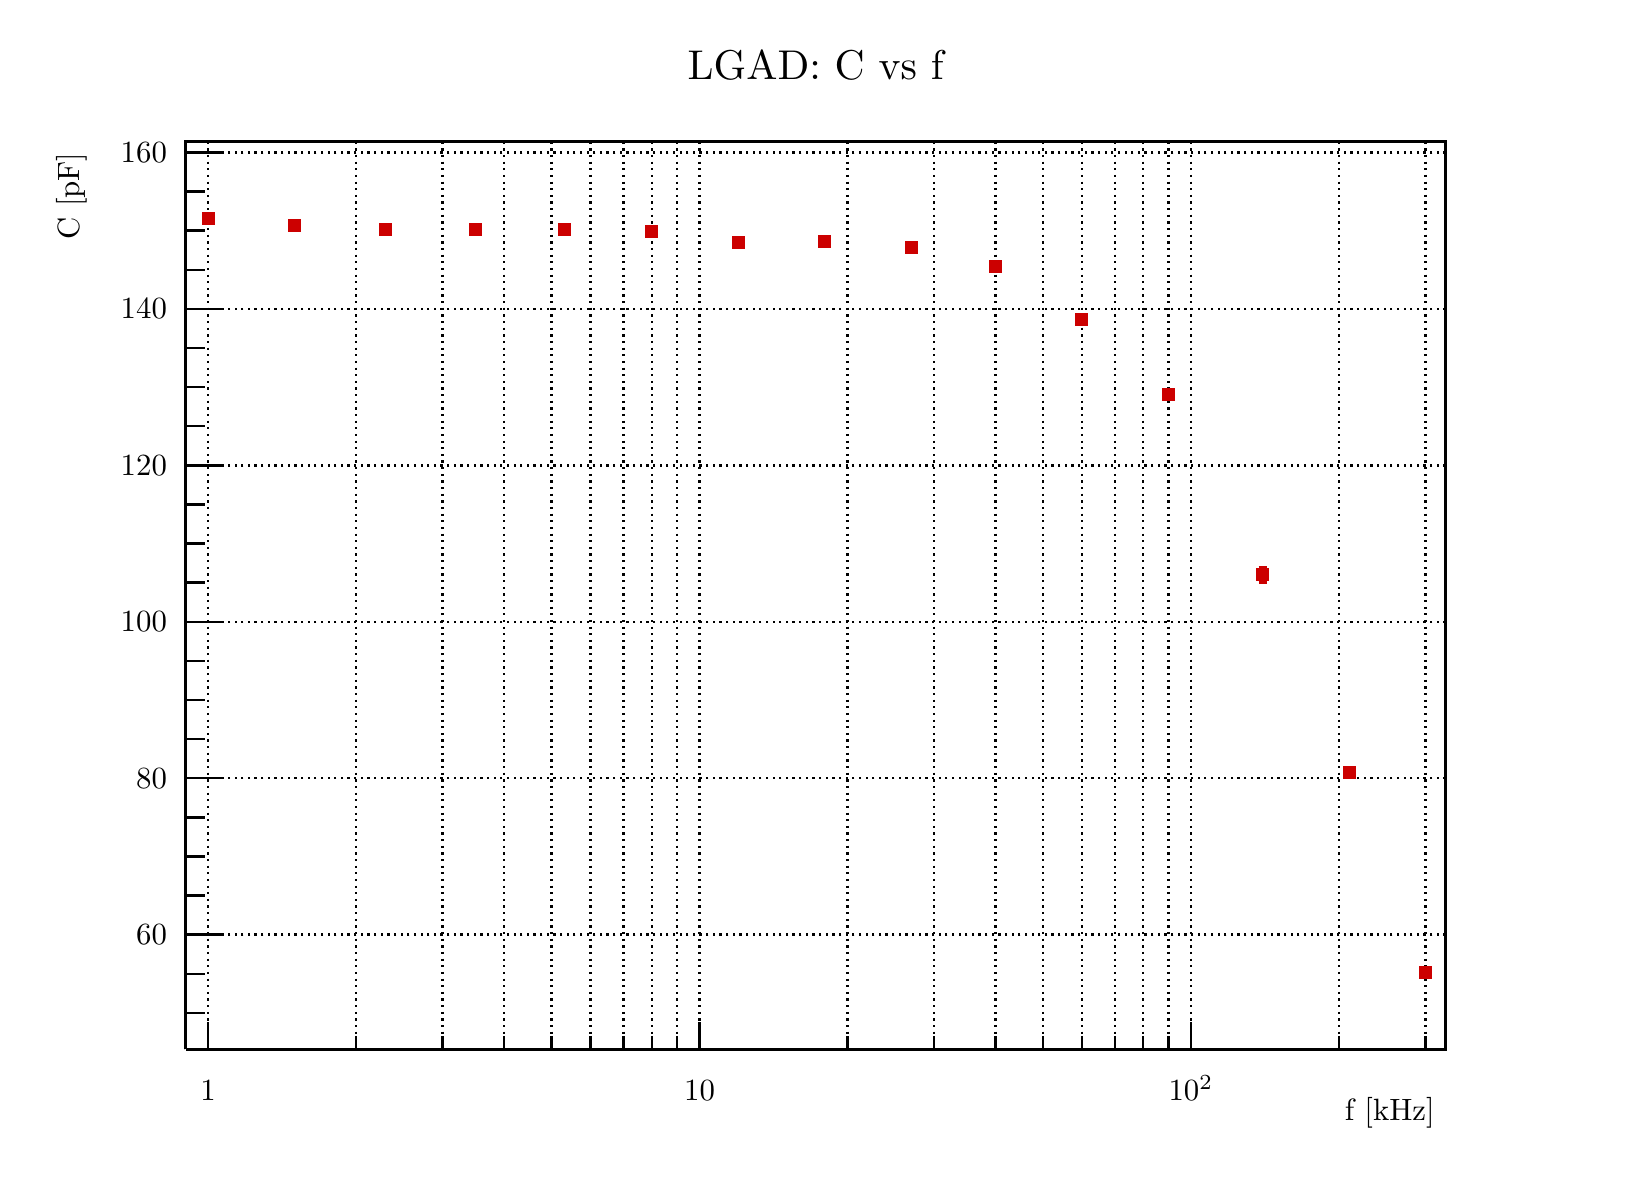
\begin{tikzpicture}
\def\CheckTikzLibraryLoaded#1{ \ifcsname tikz@library@#1@loaded\endcsname \else \PackageWarning{tikz}{usetikzlibrary{#1} is missing in the preamble.} \fi }
\CheckTikzLibraryLoaded{patterns}
\CheckTikzLibraryLoaded{plotmarks}
\pgfdeclareplotmark{cross} {
\pgfpathmoveto{\pgfpoint{-0.3\pgfplotmarksize}{\pgfplotmarksize}}
\pgfpathlineto{\pgfpoint{+0.3\pgfplotmarksize}{\pgfplotmarksize}}
\pgfpathlineto{\pgfpoint{+0.3\pgfplotmarksize}{0.3\pgfplotmarksize}}
\pgfpathlineto{\pgfpoint{+1\pgfplotmarksize}{0.3\pgfplotmarksize}}
\pgfpathlineto{\pgfpoint{+1\pgfplotmarksize}{-0.3\pgfplotmarksize}}
\pgfpathlineto{\pgfpoint{+0.3\pgfplotmarksize}{-0.3\pgfplotmarksize}}
\pgfpathlineto{\pgfpoint{+0.3\pgfplotmarksize}{-1.\pgfplotmarksize}}
\pgfpathlineto{\pgfpoint{-0.3\pgfplotmarksize}{-1.\pgfplotmarksize}}
\pgfpathlineto{\pgfpoint{-0.3\pgfplotmarksize}{-0.3\pgfplotmarksize}}
\pgfpathlineto{\pgfpoint{-1.\pgfplotmarksize}{-0.3\pgfplotmarksize}}
\pgfpathlineto{\pgfpoint{-1.\pgfplotmarksize}{0.3\pgfplotmarksize}}
\pgfpathlineto{\pgfpoint{-0.3\pgfplotmarksize}{0.3\pgfplotmarksize}}
\pgfpathclose
\pgfusepathqstroke
}
\pgfdeclareplotmark{cross*} {
\pgfpathmoveto{\pgfpoint{-0.3\pgfplotmarksize}{\pgfplotmarksize}}
\pgfpathlineto{\pgfpoint{+0.3\pgfplotmarksize}{\pgfplotmarksize}}
\pgfpathlineto{\pgfpoint{+0.3\pgfplotmarksize}{0.3\pgfplotmarksize}}
\pgfpathlineto{\pgfpoint{+1\pgfplotmarksize}{0.3\pgfplotmarksize}}
\pgfpathlineto{\pgfpoint{+1\pgfplotmarksize}{-0.3\pgfplotmarksize}}
\pgfpathlineto{\pgfpoint{+0.3\pgfplotmarksize}{-0.3\pgfplotmarksize}}
\pgfpathlineto{\pgfpoint{+0.3\pgfplotmarksize}{-1.\pgfplotmarksize}}
\pgfpathlineto{\pgfpoint{-0.3\pgfplotmarksize}{-1.\pgfplotmarksize}}
\pgfpathlineto{\pgfpoint{-0.3\pgfplotmarksize}{-0.3\pgfplotmarksize}}
\pgfpathlineto{\pgfpoint{-1.\pgfplotmarksize}{-0.3\pgfplotmarksize}}
\pgfpathlineto{\pgfpoint{-1.\pgfplotmarksize}{0.3\pgfplotmarksize}}
\pgfpathlineto{\pgfpoint{-0.3\pgfplotmarksize}{0.3\pgfplotmarksize}}
\pgfpathclose
\pgfusepathqfillstroke
}
\pgfdeclareplotmark{newstar} {
\pgfpathmoveto{\pgfqpoint{0pt}{\pgfplotmarksize}}
\pgfpathlineto{\pgfqpointpolar{44}{0.5\pgfplotmarksize}}
\pgfpathlineto{\pgfqpointpolar{18}{\pgfplotmarksize}}
\pgfpathlineto{\pgfqpointpolar{-20}{0.5\pgfplotmarksize}}
\pgfpathlineto{\pgfqpointpolar{-54}{\pgfplotmarksize}}
\pgfpathlineto{\pgfqpointpolar{-90}{0.5\pgfplotmarksize}}
\pgfpathlineto{\pgfqpointpolar{234}{\pgfplotmarksize}}
\pgfpathlineto{\pgfqpointpolar{198}{0.5\pgfplotmarksize}}
\pgfpathlineto{\pgfqpointpolar{162}{\pgfplotmarksize}}
\pgfpathlineto{\pgfqpointpolar{134}{0.5\pgfplotmarksize}}
\pgfpathclose
\pgfusepathqstroke
}
\pgfdeclareplotmark{newstar*} {
\pgfpathmoveto{\pgfqpoint{0pt}{\pgfplotmarksize}}
\pgfpathlineto{\pgfqpointpolar{44}{0.5\pgfplotmarksize}}
\pgfpathlineto{\pgfqpointpolar{18}{\pgfplotmarksize}}
\pgfpathlineto{\pgfqpointpolar{-20}{0.5\pgfplotmarksize}}
\pgfpathlineto{\pgfqpointpolar{-54}{\pgfplotmarksize}}
\pgfpathlineto{\pgfqpointpolar{-90}{0.5\pgfplotmarksize}}
\pgfpathlineto{\pgfqpointpolar{234}{\pgfplotmarksize}}
\pgfpathlineto{\pgfqpointpolar{198}{0.5\pgfplotmarksize}}
\pgfpathlineto{\pgfqpointpolar{162}{\pgfplotmarksize}}
\pgfpathlineto{\pgfqpointpolar{134}{0.5\pgfplotmarksize}}
\pgfpathclose
\pgfusepathqfillstroke
}
\definecolor{c}{rgb}{1,1,1};
\draw [color=c, fill=c] (0,0) rectangle (20,14.411);
\draw [color=c, fill=c] (2,1.4411) rectangle (18,12.9699);
\definecolor{c}{rgb}{0,0,0};
\draw [c,line width=0.9] (2,1.4411) -- (2,12.9699) -- (18,12.9699) -- (18,1.4411) -- (2,1.4411);
\definecolor{c}{rgb}{1,1,1};
\draw [color=c, fill=c] (2,1.4411) rectangle (18,12.9699);
\definecolor{c}{rgb}{0,0,0};
\draw [c,line width=0.9] (2,1.4411) -- (2,12.9699) -- (18,12.9699) -- (18,1.4411) -- (2,1.4411);
\draw [c,line width=0.9] (2,1.4411) -- (18,1.4411);
\draw [c,dash pattern=on 0.80pt off 1.60pt ,line width=0.9] (2.00001,12.9699) -- (2.00001,1.4411);
\draw [c,dash pattern=on 0.80pt off 1.60pt ,line width=0.9] (2.28553,12.9699) -- (2.28553,1.4411);
\draw [c,dash pattern=on 0.80pt off 1.60pt ,line width=0.9] (4.16393,12.9699) -- (4.16393,1.4411);
\draw [c,dash pattern=on 0.80pt off 1.60pt ,line width=0.9] (5.26272,12.9699) -- (5.26272,1.4411);
\draw [c,dash pattern=on 0.80pt off 1.60pt ,line width=0.9] (6.04233,12.9699) -- (6.04233,1.4411);
\draw [c,dash pattern=on 0.80pt off 1.60pt ,line width=0.9] (6.64704,12.9699) -- (6.64704,1.4411);
\draw [c,dash pattern=on 0.80pt off 1.60pt ,line width=0.9] (7.14112,12.9699) -- (7.14112,1.4411);
\draw [c,dash pattern=on 0.80pt off 1.60pt ,line width=0.9] (7.55886,12.9699) -- (7.55886,1.4411);
\draw [c,dash pattern=on 0.80pt off 1.60pt ,line width=0.9] (7.92073,12.9699) -- (7.92073,1.4411);
\draw [c,dash pattern=on 0.80pt off 1.60pt ,line width=0.9] (8.23991,12.9699) -- (8.23991,1.4411);
\draw [c,dash pattern=on 0.80pt off 1.60pt ,line width=0.9] (8.52544,12.9699) -- (8.52544,1.4411);
\draw [c,dash pattern=on 0.80pt off 1.60pt ,line width=0.9] (10.4038,12.9699) -- (10.4038,1.4411);
\draw [c,dash pattern=on 0.80pt off 1.60pt ,line width=0.9] (11.5026,12.9699) -- (11.5026,1.4411);
\draw [c,dash pattern=on 0.80pt off 1.60pt ,line width=0.9] (12.2822,12.9699) -- (12.2822,1.4411);
\draw [c,dash pattern=on 0.80pt off 1.60pt ,line width=0.9] (12.8869,12.9699) -- (12.8869,1.4411);
\draw [c,dash pattern=on 0.80pt off 1.60pt ,line width=0.9] (13.381,12.9699) -- (13.381,1.4411);
\draw [c,dash pattern=on 0.80pt off 1.60pt ,line width=0.9] (13.7988,12.9699) -- (13.7988,1.4411);
\draw [c,dash pattern=on 0.80pt off 1.60pt ,line width=0.9] (14.1606,12.9699) -- (14.1606,1.4411);
\draw [c,dash pattern=on 0.80pt off 1.60pt ,line width=0.9] (14.4798,12.9699) -- (14.4798,1.4411);
\draw [c,dash pattern=on 0.80pt off 1.60pt ,line width=0.9] (14.7653,12.9699) -- (14.7653,1.4411);
\draw [c,dash pattern=on 0.80pt off 1.60pt ,line width=0.9] (16.6437,12.9699) -- (16.6437,1.4411);
\draw [c,dash pattern=on 0.80pt off 1.60pt ,line width=0.9] (17.7425,12.9699) -- (17.7425,1.4411);
\draw [c,line width=0.9] (2,1.4411) -- (2,12.9699);
\draw [c,dash pattern=on 0.80pt off 1.60pt ,line width=0.9] (18,2.8986) -- (2,2.8986);
\draw [c,dash pattern=on 0.80pt off 1.60pt ,line width=0.9] (18,4.88564) -- (2,4.88564);
\draw [c,dash pattern=on 0.80pt off 1.60pt ,line width=0.9] (18,6.87268) -- (2,6.87268);
\draw [c,dash pattern=on 0.80pt off 1.60pt ,line width=0.9] (18,8.85973) -- (2,8.85973);
\draw [c,dash pattern=on 0.80pt off 1.60pt ,line width=0.9] (18,10.8468) -- (2,10.8468);
\draw [c,dash pattern=on 0.80pt off 1.60pt ,line width=0.9] (18,12.8338) -- (2,12.8338);
\draw [c,dash pattern=on 0.80pt off 1.60pt ,line width=0.9] (18,2.8986) -- (2,2.8986);
\draw [c,dash pattern=on 0.80pt off 1.60pt ,line width=0.9] (18,12.8338) -- (2,12.8338);
\draw [c,line width=0.9] (2,1.4411) -- (18,1.4411);
\draw [c,line width=0.9] (2.00001,1.61404) -- (2.00001,1.4411);
\draw [c,line width=0.9] (2.28553,1.78697) -- (2.28553,1.4411);
\draw [anchor=base] (2.28553,0.789004) node[scale=1.11327, color=c, rotate=0]{1};
\draw [c,line width=0.9] (4.16393,1.61404) -- (4.16393,1.4411);
\draw [c,line width=0.9] (5.26272,1.61404) -- (5.26272,1.4411);
\draw [c,line width=0.9] (6.04233,1.61404) -- (6.04233,1.4411);
\draw [c,line width=0.9] (6.64704,1.61404) -- (6.64704,1.4411);
\draw [c,line width=0.9] (7.14112,1.61404) -- (7.14112,1.4411);
\draw [c,line width=0.9] (7.55886,1.61404) -- (7.55886,1.4411);
\draw [c,line width=0.9] (7.92073,1.61404) -- (7.92073,1.4411);
\draw [c,line width=0.9] (8.23991,1.61404) -- (8.23991,1.4411);
\draw [c,line width=0.9] (8.52544,1.78697) -- (8.52544,1.4411);
\draw [anchor=base] (8.52544,0.789004) node[scale=1.11327, color=c, rotate=0]{10};
\draw [c,line width=0.9] (10.4038,1.61404) -- (10.4038,1.4411);
\draw [c,line width=0.9] (11.5026,1.61404) -- (11.5026,1.4411);
\draw [c,line width=0.9] (12.2822,1.61404) -- (12.2822,1.4411);
\draw [c,line width=0.9] (12.8869,1.61404) -- (12.8869,1.4411);
\draw [c,line width=0.9] (13.381,1.61404) -- (13.381,1.4411);
\draw [c,line width=0.9] (13.7988,1.61404) -- (13.7988,1.4411);
\draw [c,line width=0.9] (14.1606,1.61404) -- (14.1606,1.4411);
\draw [c,line width=0.9] (14.4798,1.61404) -- (14.4798,1.4411);
\draw [c,line width=0.9] (14.7653,1.78697) -- (14.7653,1.4411);
\draw [anchor=base] (14.7653,0.789004) node[scale=1.11327, color=c, rotate=0]{$10^{2}$};
\draw [c,line width=0.9] (16.6437,1.61404) -- (16.6437,1.4411);
\draw [c,line width=0.9] (17.7425,1.61404) -- (17.7425,1.4411);
\draw [anchor= east] (18,0.634085) node[scale=1.11327, color=c, rotate=0]{f [kHz]};
\draw [c,line width=0.9] (2,1.4411) -- (2,12.9699);
\draw [c,line width=0.9] (2.48,2.8986) -- (2,2.8986);
\draw [c,line width=0.9] (2.24,3.39536) -- (2,3.39536);
\draw [c,line width=0.9] (2.24,3.89212) -- (2,3.89212);
\draw [c,line width=0.9] (2.24,4.38888) -- (2,4.38888);
\draw [c,line width=0.9] (2.48,4.88564) -- (2,4.88564);
\draw [c,line width=0.9] (2.24,5.3824) -- (2,5.3824);
\draw [c,line width=0.9] (2.24,5.87916) -- (2,5.87916);
\draw [c,line width=0.9] (2.24,6.37592) -- (2,6.37592);
\draw [c,line width=0.9] (2.48,6.87268) -- (2,6.87268);
\draw [c,line width=0.9] (2.24,7.36944) -- (2,7.36944);
\draw [c,line width=0.9] (2.24,7.86621) -- (2,7.86621);
\draw [c,line width=0.9] (2.24,8.36297) -- (2,8.36297);
\draw [c,line width=0.9] (2.48,8.85973) -- (2,8.85973);
\draw [c,line width=0.9] (2.24,9.35649) -- (2,9.35649);
\draw [c,line width=0.9] (2.24,9.85325) -- (2,9.85325);
\draw [c,line width=0.9] (2.24,10.35) -- (2,10.35);
\draw [c,line width=0.9] (2.48,10.8468) -- (2,10.8468);
\draw [c,line width=0.9] (2.24,11.3435) -- (2,11.3435);
\draw [c,line width=0.9] (2.24,11.8403) -- (2,11.8403);
\draw [c,line width=0.9] (2.24,12.3371) -- (2,12.3371);
\draw [c,line width=0.9] (2.48,12.8338) -- (2,12.8338);
\draw [c,line width=0.9] (2.48,2.8986) -- (2,2.8986);
\draw [c,line width=0.9] (2.24,2.40184) -- (2,2.40184);
\draw [c,line width=0.9] (2.24,1.90508) -- (2,1.90508);
\draw [c,line width=0.9] (2.48,12.8338) -- (2,12.8338);
\draw [anchor= east] (1.9,2.8986) node[scale=1.11327, color=c, rotate=0]{60};
\draw [anchor= east] (1.9,4.88564) node[scale=1.11327, color=c, rotate=0]{80};
\draw [anchor= east] (1.9,6.87268) node[scale=1.11327, color=c, rotate=0]{100};
\draw [anchor= east] (1.9,8.85973) node[scale=1.11327, color=c, rotate=0]{120};
\draw [anchor= east] (1.9,10.8468) node[scale=1.11327, color=c, rotate=0]{140};
\draw [anchor= east] (1.9,12.8338) node[scale=1.11327, color=c, rotate=0]{160};
\draw [anchor= east] (0.54812,12.9699) node[scale=1.11327, color=c, rotate=90]{C [pF]};
\definecolor{c}{rgb}{0.8,0,0};
\foreach \P in {(2.28552,11.9893), (3.38432,11.9098), (4.54267,11.8502), (5.68046,11.8602), (6.80494,11.8502), (7.92072,11.8333), (9.01952,11.6913), (10.1183,11.7012), (11.2171,11.6317), (12.2822,11.3833), (13.381,10.7176), (14.4798,9.76383),
 (15.6772,7.4688), (16.776,4.95519), (17.7425,2.42171)}{\draw[mark options={color=c,fill=c},mark size=2.162162pt, line width=0.000000pt, mark=square*] plot coordinates {\P};}
\draw [c,line width=0.9] (15.6772,7.54398) -- (15.6772,7.56815);
\draw [c,line width=0.9] (15.6772,7.39361) -- (15.6772,7.36944);
\draw [c,line width=0.9] (15.627,7.56815) -- (15.7273,7.56815);
\draw [c,line width=0.9] (15.627,7.36944) -- (15.7273,7.36944);
\definecolor{c}{rgb}{0,0,0};
\draw (10,13.9427) node[scale=1.50291, color=c, rotate=0]{LGAD: C vs f};
\end{tikzpicture}
%\end{document}
